\documentclass{beamer}

% \usepackage{beamerthemesplit} // Activate for custom appearance

\usepackage[english]{babel}
\usepackage[utf8x]{inputenc}
\usepackage{amsmath}
\usepackage{graphicx}

\title{7.2 Tangent lines \& derivatives (12.1 IB SL)}
\author{Dr. Huson}
\date{\today}

\begin{document}

\frame{\titlepage}

\section[Outline]{}
\frame{\tableofcontents}

\section{Drui}
\frame
{
  \frametitle{GQ: What is the slope of a curve?}

  \begin{itemize}
  \item CCSS: Derivatives
  \item Do Now: Graph $f(x)=x^2+1$ and $y=1$\\
  \qquad (on the same graph)
  \item Lesson: Tangents to functions, derivatives (p. 200)
  \item Homework:     
  \end{itemize}
}

\section{Definition of the derivative}
\subsection{Tangent and secant}
\frame
{
  \frametitle{Definition of tangent and secant}
  \only<1>{What is the "gradient" of a curve?}
  $f(x)=x^2+1$ and $y=1$
  \begin{figure}
    \centering
    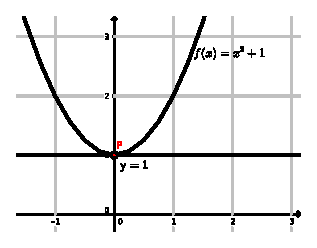
\includegraphics{7-2a-tangent.eps}
    \end{figure}
  \only<2>{
  \begin{definition}
  A \alert{secant} intersects a curve\\
  A \alert{tangent} "touches" a curve in one point (locally)
  \end{definition}}
}

\section{Definition of the derivative}
\subsection{Secant in the limit}
\frame
{
  \frametitle{Definition of the difference quotient}
  \only<1>{What is the "gradient" of the secant through points $P$ and $Q$?
  $f(x)=x^2+1$ and $y-2=m(x-1)$\qquad \qquad
  \href{https://www.geogebra.org/m/YWkaWMEQ}{link}}
  \begin{figure}
    \centering
    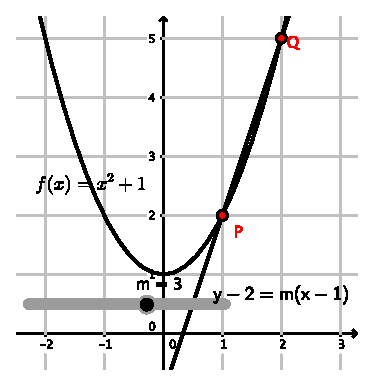
\includegraphics[height=0.4\textheight]{7-2b-secant.eps}
    \end{figure}
  \only<2>{
  Given a small $\Delta x$ from $P$ to $Q$ there will be a small change in $y$ values. The gradient will be:
  \[m=\frac {f(x+h) - f(x)}{(x+h)-h}=\frac {f(x+h) - f(x)}{h}\]
  This is called the \alert{difference quotient}}
}

\section{Definition of the derivative}
\subsection{Example slope calculation}
\frame
{
  \frametitle{Definition of the derivative}
  \only<1->{What is the "gradient" of the secant through any point $(x,f(x))$?}
  \[f(x)=x^2+1\]
  \only<2>{
  Hint: use two points on the curve, $(x,f(x))$ and $(x+h,f(x+h))$, and the slope definition:
  \[m=\frac {\Delta y}{\Delta x}\]}
  \only<3>{Substitute for $f(x)$, expand and simplify:}
  \only<3->{  \[m=\frac {\Delta y}{\Delta x}=\frac {f(x+h) - f(x)}{(x+h)-x}=\frac {((x+h)^2+1) - (x^2+1)}{h}\]}
    \only<4->{
  \[=\frac {(x^2+2xh+h^2+1) - (x^2+1)}{h}\]
  \[=\frac {2xh+h^2}{h}\]
  \[=\frac {h(2x+h)}{h}\]
  \[=2x+h\]}
  }

\section{Definition of the derivative}
\subsection{Definition of the derivative}
\frame
{
  \frametitle{Definition of the derivative}
  As $h$ gets small, the secant approaches the tangent line, and the slope approaches the local steepness of the curve at that point.
  \begin{definition}
  The \alert{derivative} of a function is the slope of a tangent line, expressed as a limit as $h$ gets very small.
  \[\lim_{h \rightarrow 0}\frac {f(x+h) - f(x)}{h}\]
  \end{definition}
  }

\section{Definition of the derivative}
\subsection{Notation}
\frame
{
  \frametitle{Definition of the derivative}
  The derivative is also called the \alert{differential} or the instantaneous rate of change, or change at the margin.\\[10pt]
  Notation:
  \[f'(x)=\lim_{h \rightarrow 0}\frac {f(x+h) - f(x)}{h}\]
  Also written as $\displaystyle \frac{dy}{dx}$ ("dee y, dee x") and $y'$ ("y prime").
  }
  
\section{Calculation of the derivative}
\subsection{Example slope calculation}
\frame
{
  \frametitle{Calculation of the derivative. Example 4 p202}
  \only<1,5->{What is the derivative of $f(x)=x^2+1$ and\\ \emph{hence} the slope of the tangent when $x=3$?}
  \only<2-4>{\[f(x)=x^2+1\]
  Definition of derivative:
  \[f'(x)=lim_{h \rightarrow 0} \frac {f(x+h) - f(x)}{h}\]}
  \only<3-4>{\[=lim_{h \rightarrow 0} \frac {((x+h)^2+1) - (x^2+1)}{h}\]}
  \only<3>{\[=lim_{h \rightarrow 0} (2x+h)\]}
  \only<4>{\[=lim_{h \rightarrow 0} (2x+h) = 2x+0\]}
  \only<4,5>{\[f'(x)=2x\]}
  \only<5>{\[f'(3) = 2(3) = 6\]}

  }
  
\end{document}